% $Header: /data/cvsroot/Courses/OnlineLearning/talks/talk4/talk4.tex,v 1.4 2006/01/24 08:08:47 yfreund Exp $

%\documentclass{beamer}
\documentclass[handout]{beamer}
%\usepackage{amsmath,latexsym,theorem}
%\usepackage[dvips]{graphicx}      %voor ps
%\usepackage[dvips]{color}

% This file is a solution template for:

% - Giving a talk on some subject.
% - The talk is between 15min and 45min long.
% - Style is ornate.

% Copyright 2004 by Till Tantau <tantau@users.sourceforge.net>.
%
% In principle, this file can be redistributed and/or modified under
% the terms of the GNU Public License, version 2.
%
% However, this file is supposed to be a template to be modified
% for your own needs. For this reason, if you use this file as a
% template and not specifically distribute it as part of a another
% package/program, I grant the extra permission to freely copy and
% modify this file as you see fit and even to delete this copyright
% notice. 


\mode<presentation>
{
  \usetheme{Montpellier}

  %\setbeamercovered{transparent}
  % or whatever (possibly just delete it)
}

\usepackage{xmpmulti} % package that defines \multiinclude

\usepackage[english]{babel}

\usepackage[latin1]{inputenc}

\usepackage{times}
\usepackage[T1]{fontenc}
% Or whatever. Note that the encoding and the font should match. If T1
% does not look nice, try deleting the line with the fontenc.

\title[Complex Expert Sets]% (optional, use only with long paper titles)
{Biased coins and the Context algorithm}

\author[Freund] % (optional, use only with lots of authors)
{Yoav Freund}
% - Give the names in the same order as the appear in the paper.
% - Use the \inst{?} command only if the authors have different
%   affiliation.

\institute[Universities of Somewhere and Elsewhere] % (optional, but mostly needed)

\subject{Machine Learning}
% This is only inserted into the PDF information catalog. Can be left
% out. 

% If you have a file called "university-logo-filename.xxx", where xxx
% is a graphic format that can be processed by latex or pdflatex,
% resp., then you can add a logo as follows:

% \pgfdeclareimage[height=0.5cm]{university-logo}{university-logo-filename}
% \logo{\pgfuseimage{university-logo}}



% Delete this, if you do not want the table of contents to pop up at
% the beginning of each subsection:
%% \AtBeginSubsection[]
%% {
%%   \begin{frame}<beamer>
%%     \frametitle{Outline}
%%     \tableofcontents[currentsection,currentsubsection]
%%   \end{frame}
%% }


% If you wish to uncover everything in a step-wise fashion, uncomment
% the following command: 

\beamerdefaultoverlayspecification{<+->}

%\newcommand{\R}[1]{{\color{red}{#1}}}
%\newcommand{\vp}{{\mathbf p}}
%\newcommand{\HedgeLoss}{L_{\mbox{\footnotesize Hedge}}}

\newcommand{\newmcommand}[2]{\newcommand{#1}{{\ifmmode {#2}\else\mbox{${#2}$}\fi}}}
\newcommand{\newmcommandi}[2]{\newcommand{#1}[1]{{\ifmmode {#2}\else\mbox{${#2}$}\fi}}}
\newcommand{\newmcommandii}[2]{\newcommand{#1}[2]{{\ifmmode {#2}\else\mbox{${#2}$}\fi}}}
\newcommand{\newmcommandiii}[2]{\newcommand{#1}[3]{{\ifmmode {#2}\else\mbox{${#2}$}\fi}}}

\newcommand{\algfnt}{\bf}

\newmcommand{\ouralg}{{\mbox{\algfnt Hedge}({\eta})}}

\newmcommand{\iter}{T}

\newfont{\cmmib}{cmmib10}
\newcommand{\boldell}{{\mbox{\cmmib \symbol{'140}}}}

\newmcommandi{\costvec}{{\boldell}^{#1}}
\newmcommandii{\cost}{{\ell}^{#1}_{#2}}

\newmcommandi{\rd}{\tilde{#1}}

\newmcommandi{\distvec}{{\bf p}^{#1}}
\newmcommandi{\rddistvec}{\rd{\bf p}^{#1}}
\newmcommandii{\dist}{{p}^{#1}_{#2}}
\newmcommandii{\rddist}{\rd{p}^{#1}_{#2}}

\newmcommandi{\bdistvec}{{\bf q}^{#1}}
\newmcommandii{\bdist}{{q}^{#1}_{#2}}

\newmcommandi{\wtvec}{{\bf w}^{#1}}
\newmcommandi{\rdwtvec}{\rd{\bf w}^{#1}}
\newmcommandii{\wt}{{w}^{#1}_{#2}}
\newmcommandii{\rdwt}{\rd{w}^{#1}_{#2}}

\newcommand{\w}[1]{\makebox[12pt]{{#1}}}
\newcommand{\Rps}{\mbox{\tt R}}
\newcommand{\rPs}{\mbox{\tt P}}
\newcommand{\rpS}{\mbox{\tt S}}
\newcommand{\rpstie}{\w{$\frac{1}{2}$}}
\newcommand{\rpswin}{\w{$0$}}
\newcommand{\rpsloss}{\w{$1$}}

\newmcommand{\decspace}{\Delta}
\newmcommand{\decsym}{\delta}
\newmcommandi{\dec}{\decsym^{#1}}
\newmcommand{\decdistsym}{\cal D}
\newmcommandi{\decdist}{{\decdistsym}^{#1}}

\newmcommand{\simpdistspace}{{\bf \cal S}}
\newmcommand{\domset}{{\rm dom}(\decdistsym)}

\newmcommand{\expdistsym}{{\cal E}}
\newmcommandii{\expdist}{{\expdistsym}^{#1}_{#2}}
\newmcommand{\expdecsym}{{\varepsilon}}
\newmcommandii{\expdec}{\expdecsym^{#1}_{#2}}

\newmcommand{\outspace}{\Omega}
\newmcommand{\outsym}{\omega}
\newmcommandi{\out}{\outsym^{#1}}

%\newmcommandii{\Dkl}{D_{\mbox{kl}}\paren{#1||#2}}
\newmcommandii{\Dkl}{{\rm {KL}}\paren{{#1}\;||\;{#2}}}

\newmcommandi{\sumwts}{\sum_{i=1}^N \wt{#1}{i}}

\newmcommand{\lossalg}{L_A}
\newmcommand{\lossouralg}{{L_{\mbox{\scriptsize\algfnt Hedge}(\eta)}}}
\newmcommand{\lossS}{{L_{\mbox{\scriptsize\algfnt S}}}}
\newmcommandi{\lossi}{L_{#1}}
\newmcommandii{\lossit}{L_{#1}^{#2}}

\newmcommandi{\upbnd}{\tilde{#1}}

\newcommand{\angles}[1]{{\left\langle {#1} \right\rangle}}
\newcommand{\paren}[1]{{\left( {#1} \right)}}
\newcommand{\abs}[1]{{\left| {#1} \right|}}
\newcommand{\ceiling}[1]{{\left\lceil {#1} \right\rceil}}

\newfont{\msym}{msbm10}
\newcommand{\real}{\mbox{\msym R}}

\newmcommand{\updatefcn}{U_\eta}

%% \newtheorem{theorem}{Theorem}	
%% \newtheorem{lemma}[theorem]{Lemma}
%% \newtheorem{corollary}[theorem]{Corollary}
%% \newtheorem{definition}{Definition}

%\newcommand{\proof}{\noindent{\bf Proof:} }
%\newcommand{\example}[1]{{\em Example #1.} }
%\newcommand{\qed}{\rule{0.7em}{0.7em}}

\newcommand{\WeakAlg}{\mbox{\algfnt WeakLearn}}
\newcommand{\Boost}{\mbox{\algfnt AdaBoost}}
\newcommand{\EX}{\mbox{\bf EX}}
\newmcommand{\hf}{h_{{f}}}
\newmcommand{\rdhf}{\rd{h}_{{f}}}
\newmcommand{\hfT}{h^T_{{f}}}
\newmcommand{\ranh}{{b}}

\newmcommand{\conclass}{{\cal C}}

\newmcommand{\badvec}{{\bf b}}
\newmcommandi{\bad}{{b}_{#1}}

%%%%%%%% New commands defined for the game-playing paper

\newmcommand{\hedge}{\algfnt Hedge}
\newmcommand{\play}{\algfnt Play}
\newmcommandi{\Glossvec}{{\bg y}^{#1}}
\newmcommandii{\Gloss}{{y}^{#1}_{#2}}
%\newmcommandi{\action}{{I}_{#1}}
\newmcommandi{\Gdistvec}{{\bf \tilde{p}}^{#1}}
\newmcommandii{\Gdist}{{\teilde{p}}^{#1}_{#2}}

%%%%%%%%%%%%%%%%%%%%%%%%%%%%%%%%%%%%%%%%%%%%%%%%%%%%%
\newmcommand{\Idistvec}{{D}}
\newmcommandi{\Idist}{\Idistvec({#1})}
\newmcommand{\Idistt}{\Idistvec_t}

\newmcommand{\Xdist}{{\cal P}}
\newmcommand{\emp}{\hat{\epsilon}}

\newmcommand{\classpc}{Y}
\newmcommand{\numclass}{k}
\newmcommandii{\prob}{\mbox{\rm Pr}_{#1}\left[{#2}\right]}
\newmcommandii{\exval}{\mbox{\rm E}_{#1}\left[{#2}\right]}

\newmcommand{\lab}{y}
\newmcommand{\ploss}{\mbox{ploss}}
\newmcommandii{\avploss}{\ploss_{#1}({#2})}
\newcommand{\sfrac}[2]{\mbox{$\frac{#1}{#2}$}}

\newcommand{\mboosta}{\mbox{\algfnt AdaBoost.M1}}
\newcommand{\mboostb}{\mbox{\algfnt AdaBoost.M2}}
\newcommand{\mboostr}{\mbox{\algfnt AdaBoost.R}}

\newmcommand{\slos}{\mbox{ploss}}
\newmcommandiii{\sloss}{\slos_{#1}({#2},{#3})}
\newmcommandiii{\avsloss}{\slos_{{#1},{#2}}({#3})}

\newmcommandii{\vwt}{{W}^{#1}_{#2}}

\newcommand{\figline}{\rule{\textwidth}{1pt}}

%\newmcommandi{\1}{{\bf 1}({#1})}
\newmcommandi{\1}{[\![{#1}]\!]}

\newmcommand{\confcn}{\kappa}
\newmcommandi{\erint}{\abs{\int_{y_i}^{h_t(x_i)} {#1} dy}}
%\newmcommandi{\erint}{\int_{\min\{y_i,h_t(x_i)\}}^{\max\{y_i,h_t(x_i)\}}{#1}dy}

\newcommand{\blue}[1]{{\color{blue}{#1}}}
\newcommand{\red}[1]{{\color{red}{#1}}}
\newcommand{\redEq}[1]{{\color{red}{$#1$}}}
\newcommand{\W}{\vec{W}}
\newcommand{\V}{\vec{V}}
\newcommand{\X}{\vec{X}}
\newcommand{\loss}{\vec{\ell}}
\newcommand{\HedgeLoss}{L_{\mbox{\footnotesize Hedge}}}


\begin{document}

%\iffalse %%%%%%%%%%%%%%%%%%%%%%%%%%%%%%%%%%%%%%%%%%%%%%%%%%%%%%%%%%%%%%%%%%

\begin{frame}
  \titlepage
\end{frame}

\begin{frame}
  \frametitle{Outline}
  \tableofcontents[pausesections]
  % You might wish to add the option [pausesections]
\end{frame}

\section{Combining experts in the log loss framework}

\begin{frame}
\frametitle{The log-loss framework}
\begin{itemize}
\item Algorithm \R{$A$} predicts a sequence \R{$c^1,c^2,\ldots, c^T$}
over alphabet \R{$\Sigma = \{1,2,\ldots,k\}$}
\item The prediction for the \R{$c^t$}th is a distribution over \R{$\Sigma$}:\\
\R{$\vp_A^t = \langle p_A^t(1),p_A^t(2),\ldots,p_A^t(k) \rangle$} 
\item When $c^t$ is revealed, the loss we suffer is \R{$-\log p_A^t(c^t)$}
\item The {\color{blue}cumulative log loss}, which we wish to minimize, 
is \R{$\lossalg^T = -\sum_{t=1}^T \log p_A^t(c^t)$}
\item \R{$\lceil \lossalg^T \rceil$} is the code length if \R{$A$} is combined with arithmetic coding.
\end{itemize}
\end{frame}

\begin{frame}
\frametitle{The game}
\begin{itemize}
\item Prediction algorithm \R{$A$} has access to \R{$N$} experts.
\item The following is repeated for \R{$t=1,\ldots,T$}
\begin{itemize}
\item Experts generate predictive distributions: \R{$\vp_1^t,\ldots,\vp_N^t$}
\item Algorithm generates its own prediction \R{$\vp_A^t$}
\item \R{$c^t$} is revealed.
\end{itemize}
\item {\bf Goal:} minimize regret:
\R{\[
-\sum_{t=1}^T \log p_A^t(c^t) + \min_{i=1,\dots,N} \paren{-\sum_{t=1}^T \log p_i^t(c^t)} 
\]}
\end{itemize}
\end{frame}

\section{The online Bayes Algorithm}

\begin{frame}
\frametitle{The online Bayes Algorithm}
\begin{itemize}
\item {\color{blue} Total loss} of expert \R{$i$}
\R{$$L_i^t = - \sum_{s=1}^{t} \log p_i^s(c^s);\;\;\; L_i^0 = 0$$}
\item {\color{blue}Weight} of expert \R{$i$}
\R{$$\wt{t}{i} = \wt{1}{i} e^{-L_i^{t-1}} = \wt{1}{i} \prod_{s=1}^{t-1} p_i^s(c^s)$$}
\item
Freedom to choose initial weights.\\
 \R{$\wt{1}{t} \geq 0$}, \R{$\sum_{i=1}^n \wt{1}{i} = 1$}
\item {\color{blue}Prediction} of algorithm \R{$A$}
\R{\[
\vp_A^t = \frac{\sum_{i=1}^N \wt{t}{i} \vp_i^t}{\sum_{i=1}^N \wt{t}{i}}
\]}
\end{itemize}
\end{frame}

\section{The performance bound}
%\fi %%%%%%%%%%%%%%%%%%%%%%%%%%%%%%%%%%

\begin{frame}
\frametitle{Cumulative loss vs. Final total weight}

\onslide<1-> Total weight: \R{$W^t \doteq \sum_{i=1}^N \wt{t}{i}$}

\onslide<2-> \R{$$
\frac{W^{t+1}}{W^t}  =  \frac{\sum_{i=1}^N \wt{t}{i} e^{\log p_i^t(c^t)}}{\sum_{i=1}^N \wt{t}{i}} 
\onslide<3->          =   \frac{\sum_{i=1}^N \wt{t}{i} p_i^t(c^t)}{\sum_{i=1}^N \wt{t}{i}} 
\onslide<4->        =  p_A^t(c^t)
$$}
\onslide<5-> \R{$$ -\log \frac{W^{t+1}}{W^t} = -\log p_A^t(c^t) $$}
\R{\[
\onslide<8-> -\log W^{T+1} =
\onslide<6-> -\log \frac{W^{T+1}}{W^1} = -\sum_{t=1}^T \log p_A^t(c^t)
\onslide<7-> = L_A^T
\]}
\onslide<9-> \R{\bf EQUALITY} not bound!
\end{frame}

\begin{frame}
\frametitle{Simple Bound}
\begin{itemize}
\item Use uniform initial weights \R{$\wt{1}{i} = 1/N$}
\item Total Weight is at least the weight of the best expert.
\R{\begin{eqnarray*}
L_A^T & = & -\log W^{T+1} 
\pause = -\log \sum_{i=1}^N \wt{T+1}{i} \\
\pause & = & -\log \sum_{i=1}^N \frac{1}{N} e^{-L_i^T} 
\pause  =  \log N - \log \sum_{i=1}^N e^{-L_i^T}\\
\pause & \leq & \log N - \log \max_i e^{-L_i^T}  
\pause = \log N + \min_i L_i^T
\end{eqnarray*}}
\item Dividing by $T$ we get
\R{$ \frac{L_A^T}{T} = \min_i \frac{L_i^T}{T} + \frac{\log N}{T} $}
\end{itemize}
\end{frame}


\begin{frame}
\frametitle{Bound better than for two part codes}
\begin{itemize}
\item
Simple bound as good as bound for two part codes (MDL) 
but enables online compression
\item Suppose we have \R{$K$} copies of each expert.
\item Two part code has to point to one of the $KN$ experts
\R{$ L_A \leq \log NK + \min_i L_i^T = \log NK + \min_i L_i^T$}
\item If we use Bayes predictor + arithmetic coding we get:
\R{$$ L_A = -\log W^{T+1} \leq \log  K \max_i \frac{1}{NK} e^{-L_i^T} 
=\log N + \min_i L_i^T $$}
\item We don't pay a penalty for copies.
\item More generally, the regret is smaller if many of the experts perform well.
\end{itemize}
\end{frame}


\section{Comparison with Bayesian Statistics}

\begin{frame}
\frametitle{Comparison with standard Bayesian statistics}
\begin{itemize}
\item The weight update rule is the same.
\item Normalized weights $=$ {\bf posterior probability  distribution}.
\item Bayesian analysis interested in the {\bf final} posterior.
\item Bayesian analysis assumes the data is {\bf generated} 
by a distribution in the support of the prior.
\item Goal of Bayesian is to {\bf estimate true distribution}, 
goal of online learning is to {\bf minimize regret}.
\item Optimality of algorithm is {\bf axiom} of Bayesian statistics.
\item Bayesian methods perform poorly when the loss is not log loss
  and the data not generated by a distribution in the support.
\begin{itemize}
\item
Loss can sometimes be defined through the noise distribution: square loss is equivalent to assuming guassian noise.
\item
For number of mistakes - Bayesian method cannot be ``fixed''. Requires variable learning rate.
\end{itemize}
\end{itemize}
\end{frame}

% \section{Least Informative Priors}

\section{Computational issues}

\begin{frame}
\frametitle{Computational Issues}
\begin{itemize}
\item Naive implementation: calculate the prediction of each of 
the \R{$N$} experts.
\item Puts severe limit on number of experts.
\item What if set of experts is uncountably infinite.
\item Bayesian tricks:
\begin{itemize}
\item {\bf Conjugate priors}: A prior over a continuous domain whose functional form does not change with when updated. 
\pause Number of parameters defining posterior is constant. 
\pause Update rule translates into update of parameters.
\pause parameters correspond to ``sufficient statistics''.
\pause exists for the familty of exponential distributions.
\item {\bf Markov Chain Monte Carlo} Sample the posterior. 
\pause Can sometimes be done efficiently.
\pause Efficient sampling relates to mixing rate of markov chain whose limit dist is the posterior dist. 
\end{itemize}
\end{itemize}
\end{frame}

\section{The Universal prediction machine}

\begin{frame}
\frametitle{Standardizing online prediction algorithms}
\begin{itemize}
\item Fix a universal Turing machine \R{$U$}.
\item An online prediction algorithm \R{$E$} is a program that 
\begin{itemize}
\item
given as input {\color{blue} The past} \R{$\X \in \{0,1\}^t$}
\item runs finite time and outputs
\item
A prediction for the next bit \R{$p(\X) \in [0,1]$}.
\item 
To ensure \R{$p$} has a finite description. Restrict to {\color{blue}rational} numbers 
\R{$n/m$}
\end{itemize}

\item \B{Any} online prediction algorithm can be represented as code \R{$\vb(E)$}
for \R{$U$}. The code length is \R{$|\vb(E)|$}.
\item Most sequences do not correspond to valid prediction algorithms. 
\item 
\R{$V(\vb,\X,t)=1$} if the program \R{$\vb$}, given \R{$\X$} as input, 
halts within \R{$t$} steps and outputs a well-formed prediction. Otherwise \R{$V(\vb,\X,t)=0$}
\item \R{$V(\vb,\X,t)$} is computable (recursively enumerable).
\end{itemize}
\end{frame}

\begin{frame}
\frametitle{A universal prediction machine}
\begin{itemize}
\item Assign to the code \R{$\vb$} the initial weight \R{$\wt{1}{\vb} = 2^{-|\vb|-\log_2 |\vb|}$}.
\item The total initial weight over all finite binary sequences is one.
\item Run the Bayes algorithm over ``all'' prediction algorithms.
\item \B{technical details:} On iteration \R{$t$}, \R{$|\X|=t$}. 
Use the predictions of 
programs \R{$\vb$} such that \R{$|\vb| \leq t$} and for which \R{$V(\vb,\X,2^t)=1$}. Assing the remaining mass the prediction \R{$1/2$} (insuring a loss of \R{$1$})
\end{itemize}
\end{frame}

\begin{frame}
\frametitle{Performance of the universal prediction algorithm}
\begin{itemize}
\item Using \R{$ L_A \leq \min_i \paren{ L_i -\log \wt{1}{i}}$}
\item Assume \R{$E$} is a prediction algorithm which generates the 
\R{$t$}th prediction in time smaller than \R{$2^t$}
\item When \R{$t \leq |\vb(E)|$} the algorithm is not used and thus it's loss is \R{$1$}
\item We get that the loss of the Universal algorithm is at most 
\R{$2|\vb(E)| + \log_2 |\vb(E)| + L_E$}
\item More careful analysis can reduce \R{$2|\vb(E)| + \log_2 |\vb(E)|$} to \R{$|\vb(E)|$}
\item Code length is arbitrarily close to the Kolmogorov Complexity of the sequence.
\item Ridiculously bad running time.
\end{itemize}
\end{frame}

\begin{frame}
\frametitle{Bayes coding is better than two part codes}
\begin{itemize}
\item
Simple bound as good as bound for two part codes (MDL) 
but enables online compression
\item Suppose we have \R{$K$} copies of each expert.
\item Two part code has to point to one of the $KN$ experts
\R{$ L_A \leq \log NK + \min_i L_i^T = \log NK + \min_i L_i^T$}
\item If we use Bayes predictor + arithmetic coding we get:
\R{$$ L_A = -\log W^{T+1} \leq \log  K \max_i \frac{1}{NK} e^{-L_i^T} 
=\log N + \min_i L_i^T $$}
\item We don't pay a penalty for copies.
\item More generally, the regret is smaller if many of the experts perform well.
\end{itemize}
\end{frame}

\section{The biased coins set of experts}
\begin{frame}
\frametitle{The biased coins set of experts}
\begin{itemize}
\item Each expert corresponds to a biased coin, predicts with a fixed \R{$\theta \in [0,1]$}.
\item Set of experts is \R{uncountably infinite}.
\item Only countably many experts can be assigned non-zero weight.
\item Instead, we assign the experts a \R{Density Measure}.
\item \R{$ L_A \leq \min_i \paren{ L_i -\log \wt{1}{i}}$} is meaningless.
\item Can we still get a meaningful bound?
\end{itemize}
\end{frame}

%\subsection{Bayes using Jeffrey's prior}

\begin{frame}
\frametitle{Bayes Algorithm for biased coins}
\begin{itemize}
\item 
Replace the initial weight by a density measure \R{$\dweight{\theta}{} =
\dweight{\theta}{1}$, $\int_0^1 \dweight{\theta}{} d\theta=1$}
\item 
Relationship between final total weight and total log loss remains unchanged:
\R{\[
 \TAloss = \ln \int_0^1 \dweight{\theta}{} e^{-\TEloss{\theta}^{T+1}} d\theta
\]}
\item
We need a new \B{lower bound} on the final total weight
\end{itemize}
\end{frame}

 \begin{frame}
\frametitle{Main Idea}
If \R{$\dweight{\theta}{t}$} is large then \R{$\dweight{\theta+\epsilon}{t}$} is also large.
~\pause
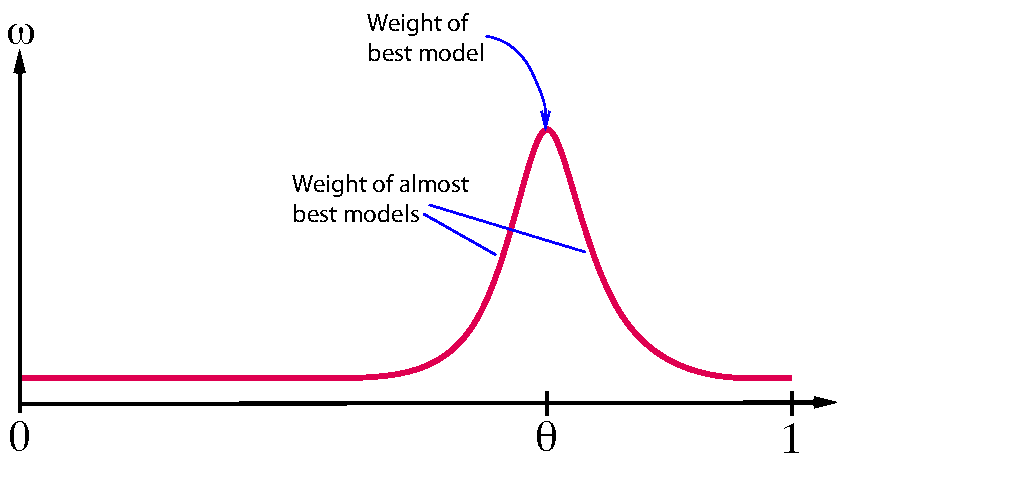
\includegraphics[height=6cm]{figures/neighborhood.pdf}
\end{frame}

%\subsection{Laplace Approximation}
\begin{frame}
\frametitle{Expanding the exponent around the peak}

\begin{itemize}
\item
For log loss the best \R{$\theta$} is empirical distribution
of the seq.
\R{\[
	\btheta = {\#\{x^t=1;\;\; 1 \leq t \leq T \} \over T} 
\]}
\item
The total loss scales with \R{$T$}
\R{\[
\TEloss{\theta} =
 T \cdot (\btheta \ell(\theta,1) + (1-\btheta)\ell(\theta,0))
 \doteq T \cdot g(\btheta,\theta)
\]}
\end{itemize}
\pause
\R{ \begin{eqnarray*}
\TAloss - \BEloss &\leq&
\ln \int_0^1 \dweight{\theta}{} e^{- \TEloss{\theta}} d\theta
- \ln e^{\BEloss} \\
\pause &=&
\ln \int_0^1 \dweight{\theta}{} e^{-
(\TEloss{\theta}-\BEloss)} d\theta \\
\pause &=&
\ln \int_0^1 \dweight{\theta}{} 
e^{T (g(\btheta,\theta) - g(\btheta,\btheta))} d\theta
\end{eqnarray*}}
\end{frame}

\begin{frame}
\frametitle{Laplace approximation (idea)}
\begin{itemize}
\item Taylor expansion of \R{$g(\btheta,\theta)-g(\btheta,\btheta)$} around \R{$\theta=\btheta$}.
\item
First and second terms in the expansion are zero.
\item
Third term gives a quadratic expression in the exponent
\item
$\Rightarrow$ a gaussian approximation of the posterior.
\end{itemize}
\pause
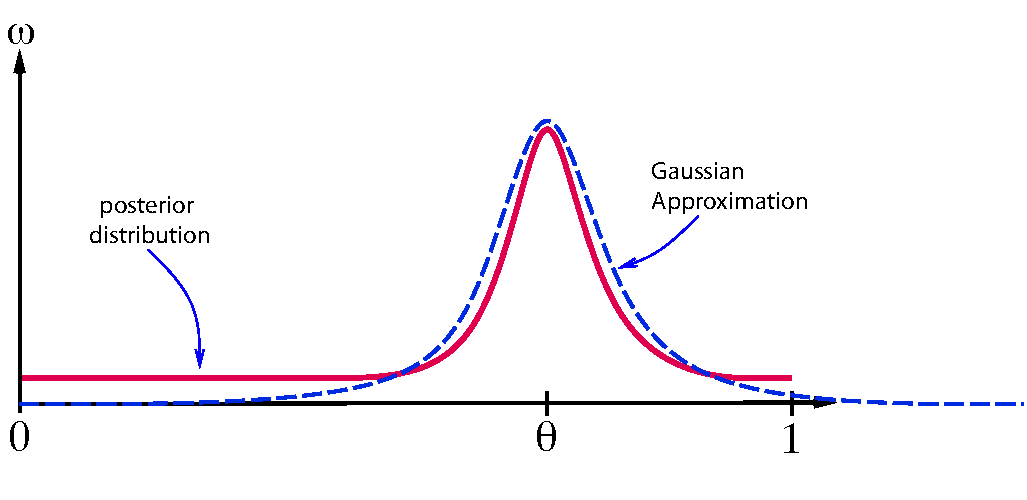
\includegraphics[height=5cm]{figures/Laplace.pdf}

\end{frame}

\begin{frame}
\frametitle{Laplace Approximation (details)}

\R{\begin{eqnarray*}
\lefteqn{\int_0^1  \dweight{\theta}{} 
         e^{T (g(\btheta,\theta)-g(\btheta,\btheta))} d\theta}\\
\pause &=& \dweight{\btheta}{} \sqrt{-2 \pi \over 
T \left. {d^2 \over d\theta^2} \right|_{\theta=\btheta} 
(g(\btheta,\theta)-g(\btheta,\btheta))}
+ O(T^{-3/2})
\end{eqnarray*}}
\end{frame}

%\subsection{Choosing the optimal prior}

\begin{frame}
\frametitle{Choosing the optimal prior}
\begin{itemize}
\item
Choose \R{$\dweight{\theta}{}$} to maximize the worst-case final total weight
\R{\[
\min_{\btheta} \dweight{\btheta}{} \sqrt{-2 \pi \over 
T \left. {d^2 \over d\theta^2} \right|_{\theta=\btheta} 
(g(\btheta,\theta)-g(\btheta,\btheta))}
\]}
\item
Make bound equal for all \R{$\btheta \in [0,1]$} by choosing
\R{\[
\dweight{\btheta}{*} =
{1 \over Z}
\sqrt{\left. {d^2 \over d\theta^2} \right|_{\theta=\btheta} 
(g(\btheta,\theta)-g(\btheta,\btheta)) \over - 2 \pi}~,
\]}
where \R{$Z$} is the normalization factor:
\R{\[
Z =\sqrt{1 \over 2 \pi}\;\;
\int_0^1 \;\;\sqrt{\left. {d^2 \over d\theta^2} \right|_{\theta=\btheta} 
(g(\btheta,\btheta)-g(\btheta,\theta))} \;\;d\btheta
\]}
\end{itemize}
\end{frame}


\begin{frame}
\frametitle{The bound for the optimal prior}
\begin{itemize}
\item Plugging in we get
\R{\begin{eqnarray*}
\TAloss - \BEloss &\leq&
\ln \int_0^1 \dweight{\theta}{*} 
e^{T (g(\btheta,\theta) - g(\btheta,\btheta))} d\theta \\
&=&
\ln \left( \sqrt{2\pi Z \over T} + O(T^{-3/2}) \right) \\
&=&
{1 \over 2} \ln {T \over 2\pi} -{1 \over 2} \ln Z + O(1/T)~.
\end{eqnarray*}}
\end{itemize}
\end{frame}

\begin{frame}
\frametitle{Solving for log-loss}
\begin{itemize}
\item
The exponent in the integral is
\R{\[
g(\btheta,\theta) - g(\btheta,\btheta)
=
\btheta \ln {\btheta \over \theta} + 
(1-\btheta) \ln {1-\btheta \over 1-\theta}
=
D_{KL} (\btheta || \theta)
\]}
\item
The second derivative
\R{\[
\left. {d^2 \over d\theta^2} \right|_{\theta=\btheta} 
D_{KL} (\btheta || \theta) = \btheta (1-\btheta)
\]}
Is called the \B{empirical Fisher information}
\item
The optimal prior:
\R{\[
\dweight{\btheta}{*} = \frac{1}{\pi \sqrt{\btheta (1-\btheta)}}
\]}
Known in general as \B{Jeffrey's prior}.  And, in this case, 
the \B{Dirichlet-$(1/2,1/2)$ prior}.
\end{itemize}
\end{frame}

\begin{frame}
\frametitle{The cumulative log loss of Bayes using Jeffrey's prior}
\begin{itemize}
\item
\R{\[
\TAloss - \BEloss \leq {1 \over 2} \ln (T+1) 
                     + {1 \over 2} \ln {\pi \over 2}
                     + O(1/T)
\]}
\end{itemize}
\end{frame}

%\subsection{Kritchevski Trofimov Prediction Rule}
\begin{frame}
\frametitle{But what is the prediction rule?}
\begin{itemize}
\item As luck would have it the Dirichlet prior is the \B{conjugate prior} for the Binomial distribution.
\item
Observed \R{$t$} bits, \R{$n$} of which were \R{$1$}. The posterior is:
\R{\[
\frac{1}{Z \sqrt{\theta(1-\theta)}} \theta^n (1-\theta)^{t-n} 
 = 
\frac{1}{Z} \theta^{n-1/2} (1-\theta)^{t-n-1/2} 
\]}
\item
The posterior average is:
\R{\[
\frac{\int_0^1 \theta^{n+1/2} (1-\theta)^{t-n-1/2} d\theta}
{\int_0^1 \theta^{n-1/2} (1-\theta)^{t-n-1/2} d\theta}
=
\frac{n+1/2}{t+1}
\]}
\item This is called the Trichevsky Trofimov prediction rule.
\end{itemize}
\end{frame}

%\subsection{Laplace Rule of Succession}
\begin{frame}
\frametitle{Laplace Rule of Succession}
\begin{itemize}
\item
Laplace suggested using the uniform prior, which is also a conjugate prior.
\item In this case the posterior average is:
\R{\[
\frac{\int_0^1 \theta^{n+1} (1-\theta)^{t-n} d\theta}
{\int_0^1 \theta^{n} (1-\theta)^{t-n} d\theta}
=
\frac{n+1}{t+2}
\]}
\item
The bound on the cumulative log loss is worse:
\R{\[
\TAloss - \BEloss = \ln T + O(1)
\]}
\item
Suffers larger regret when \R{$\btheta$} is far from \R{$1/2$}
\end{itemize}
\end{frame}

%\section{Priors for finite $t$}

%\section{Shtarkov lower bound for finite horizon}

\begin{frame}
\frametitle{Shtarkov Lower bound}
\begin{itemize}
\item What is the \B{optimal} prediction when \R{$T$} is know in
  advance?
\item
\R{\[
L_*^T - \min_\theta L_\theta^T \geq \frac{1}{2} \ln(T+1) + \frac{1}{2}
\ln \frac{\pi}{2} - O(\frac{1}{\sqrt{T}})
\]}
\end{itemize}
\end{frame}

\section{Generalization to larger sets of distributions}

\begin{frame}
\frametitle{Multinomial Distributions}
\begin{itemize}
\item For a distribution over \R{$k$} elements (Multinomial) \B{[Xie and Barron]}
\item Use the add 1/2 rule (KT).
\R{\[
p(i) = \frac{n_i+1/2}{t+k/2}
\]}
\item Bound is
\R{\[\TAloss - \BEloss \leq \frac{k-1}{2}\ln T + C + o(1)\]}
\item 
The constant C is optimal.
\end{itemize}
\end{frame}

\begin{frame}
\frametitle{Exponential Distributions}
\begin{itemize}
\item For any set of distributions from the exponential family
  defined by \R{$k$} parameters (constituting an open set) \B{[Rissanen96]}
\item Use Bayes Algorithm with Jeffrey's prior:
\R{\[
\dweight{\btheta}{*} = \frac{1}{Z} 
\frac{1}{\sqrt{
\left| \left. {\mathbf H} \paren{D_{KL} (\btheta || \theta) } \right|_{\theta=\btheta} \right|
}}
\]}
\R{$\mathbf H$} denotes the Hessian.
\item
\R{\[\TAloss - \BEloss \leq \frac{k-1}{2}\ln T - \ln Z + o(1)\]}
\end{itemize}
\end{frame}

\begin{frame}
\frametitle{General Distributions}
\begin{itemize}
\item Characterize distribution family by metric entropy.
\item Fixed parameter set usually corresponds to polynomial metrix
  entropy
\R{ \[
N(1/\epsilon) = O\paren{\frac{1}{\epsilon^d}}
\]}
\R{$d$} is the number of parameters.
\item
\B{[Haussler and Opper]} show that the coefficient in front of \R{$\ln
  T$} is optimal for distribution families where the metric entropy is
  up to 
\R{\[ 
N(1/\epsilon) = O\paren{e^{\epsilon^{-\alpha}}}
\]}
For all \R{$\alpha \leq 5/2$}.
\end{itemize}
\end{frame}

\section{Fixed Length Markov Models}

%An Example
\begin{frame}
\frametitle{A fixed length Markov Model}
\begin{columns}
\begin{column}[t]{8cm}
\begin{itemize}
\item Observe a binary sequence.
\item \R{$x_1,\ldots,x_{t-1}$}
\item Predict next bit from past
\item \R{$P(x_t=1 | x_{t-1},x_{t-2},\ldots,x_1)$}
\item Use only last \R{$k$} bits
\item \R{$P(x_t=1 | x_{t-1},\ldots,x_{t-k})$}
\item Markov model of order \R{$k$}
\end{itemize}
\end{column}
\begin{column}[T]{5cm}
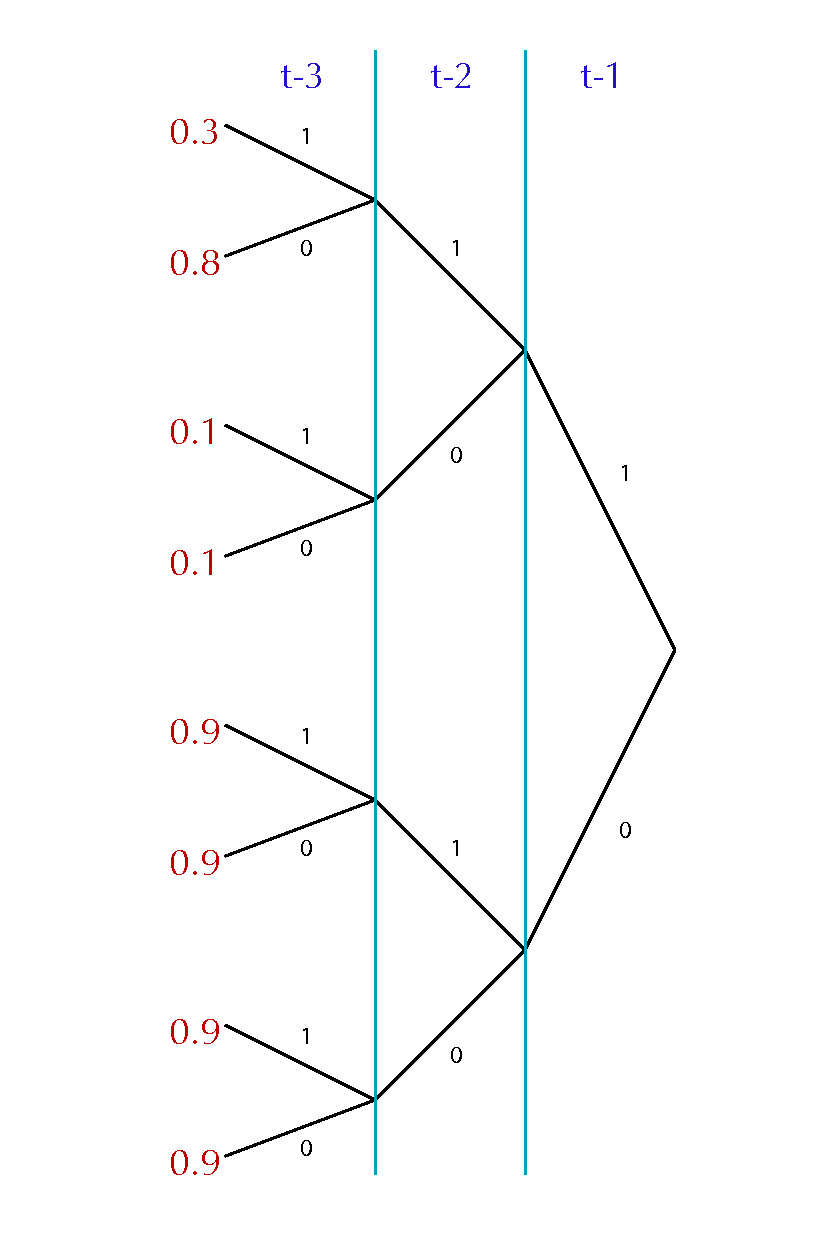
\includegraphics[width=4.5cm]{figures/PredictionTree.pdf}
\end{column}
\end{columns}
\end{frame}

%Using the KT predictor in each element
\begin{frame}
\frametitle{Learning a markov distribution}
\begin{itemize}
\item Each tree leaf is associated with a binary sequence
\R{$y_1,\ldots,y_k$} 
\item For each leaf keep two counters:
\begin{itemize}
\item \R{$a_{y_1,\ldots,y_k}$} = number of times \R{$x_{t-1}=y_1, \ldots, x_{t-k}=y_k$} \\ and \R{$x_t=0$}
\item \R{$b_{y_1,\ldots,y_k}$} = number of times \R{$x_{t-1}=y_1, \ldots, x_{t-k}=y_k$} \\ and \R{$x_t=1$}
\end{itemize}
\item Prediction (using Kritchevski Trofimov)
\R{\[p(x_t=1 | x_{t-1}=y_1,\ldots,x_{t-k}=y_k) 
= \frac{b_{y_1,\ldots,y_k}+1/2}{a_{y_1,\ldots,y_k}+b_{y_1,\ldots,y_k}+1}\]}
\item Total regret is at most \R{$2^{k-1} \log T$}
\end{itemize}
\end{frame}

\section{Variable Length Markov Model (VMM)}

%Why variable length is better than fixed length. (QU example)

\begin{frame}
\frametitle{How variable length markov can reduce regret}
\begin{columns}
\begin{column}[T]{5cm}
\multiinclude[graphics={width=4.5cm},format=pdf]{figures/PredictionTree}
\end{column}
\begin{column}[t]{8cm}
\begin{itemize}
\item Reducing number of leaves from \R{$8$} to \R{$4$} means 
\item reducing regret from \R{$4 \log T$} to \R{$2 \log T$}
\item English example: \\
\B{B \pause A \pause R \pause O \pause Q }\pause \R{U} \pause \B{E}
\item When we have little data, we can get better prediction even if the children are not 
\B{Exactly the same}
\end{itemize}
\end{column}
\end{columns}
\end{frame}

%defining complete trees
\begin{frame}
\frametitle{Prefix trees}
\begin{itemize}
\item In a prefix binary tree each node has either \R{0} or \R{2} children.
\item A node with \R{1} child means that some past histories are not covered.
\item A variable length markov model corresponds to a \B{prefix tree}.
\item But we don't know which prefix tree to use!
\end{itemize}
\end{frame}

\begin{frame}
\frametitle{Assigning probabilities to complete sequences}
\begin{itemize}
\item Using the chain rule, we can use a prediction rule to 
assign probabilities to a complete sequence.
\R{\[
P \paren{x_1=y_1,\ldots,x_T=y_T} = p \paren{x_1=y_1} p\paren{x_2=y_2|x_1=y_1} \ldots
\]}
\item
We can translate probabilities for complete sequences back into predictions.
\R{\begin{eqnarray*}
p \paren{ x_t=1 | x_1=y_1,\ldots,x_{t-1}=y_{t-1}} = \\
\frac{p\paren{x_1=y_1,\ldots,x_{t-1}=y_{t-1},x_t=1}}
{p\paren{x_1=y_1,\ldots,x_{t-1}=y_{t-1}}}
\end{eqnarray*}}
\item
Will come in handy soon!
\end{itemize}
\end{frame}

\section{Assigning weights to trees}

% Using bayesian method to perform almost as well as the best VMM
\section{Learning the structure, an inefficient solution}

\begin{frame}
\frametitle{Using online Bayes to learn the structure}
\begin{itemize}
\item We assign to each tree an initial weight of \R{$2^{-n}$} where \R{$n$} is the number of \B{nodes} in the 
prefix tree.
\item We combine the predictions of the trees using online Bayes.
\item The total regret would be \R{$\frac{l}{2}\log T + n$} where \R{$l$} is the number of \B{leaves} in the prefix tree.
\item The papers do things slightly differently because they bound the depth of the tree by \R{$k$}.
\item This algorithm maintains a weight for each tree.
\item Requires maintaining \R{$O(2^l)$} weights!
\end{itemize}
\end{frame}

% Defining the distribution using a random process.

\section{Efficient Implementation}

\begin{frame}
\frametitle{Efficient implementation}
\begin{itemize}
\item \B{First idea:} Estimate probabilities of complete sequences and use conditional to generate predictions.
\item The prior weights are used for averaging the complete sequence probabilities - they don't need to be updated.
\item \B{Second idea:} Compute the average over the prior efficiently.
\end{itemize}
\end{frame}

\begin{frame}
\frametitle{Efficient generation of prior}
\begin{itemize}
\item Prior distribution is generated by a stochastic recursion.
\item Start with root node (always exists)
\item For each node flip a fair coin.
\begin{itemize}
\item \B{Heads} Set node to be a leaf (\R{0} children)
\item \B{Tails} Create \R{2} children nodes to the node.
\end{itemize}
\item Defines a distribution over all prefix trees.
\item Probability of a tree with \R{$n$} nodes is \R{$2^{-n}$}
\end{itemize}
\end{frame}

% computing the posterior takes linear time because we can use the
% random process definition.
\begin{frame}
\frametitle{Efficient averaging over the prior (observations)}
\begin{itemize}
\item Maintain a KT estimator at each node of the tree.
\item Allocate counters only once node is visited.
\item At iteration \R{$t$} only \R{$t$} counters need to be updated.
\item Only \R{$k$} counters if depth of tree is bounded.
\item Each node is visited on a subset of the iterations.
\item Subset corresponding to node is contained in subset corresponding to node's parent.
\end{itemize}
\end{frame}

% Updating the weights takes linear time
\begin{frame}
\frametitle{Efficient averaging over the prior (procedure)}
\begin{itemize}
\item \R{$P_e\paren{a_s,b_s}$} the probability that the KT estimator at node 
\R{$s=\left\langle y_1,..,y_k \right\rangle$} assigns to it's subsequence of the past.
\item \R{$P_w^s$} the \B{average probability} assigned to the subsequence \B{over all VMM rooted} at the node \R{$s$}
\item
\R{\[
P_w^s \doteq 
\frac{P_e \paren{a_s,b_s} + P_w^{0s}P_w^{1s}}{2}
\]}
\item Average probability assigned by the complete tree is \R{$P_w^\lambda$} where \R{$\lambda$} is the root node.
\end{itemize}
\end{frame}

%%%%%%%%%%%%%%%%%%%%%%%%%%%%%%%%%%%%%%%%%%%%%%%%%%%%%%%%%%%%%%%%%%%%%%%%%%
\begin{frame}
\begin{center}
{\bf\Large Context-Tree Weighting and Maximizing: Processing Betas}
\\
\vspace{10mm}
{Frans Willems, Tjalling Tjalkens, and Tanya Ignatenko,\\
Eindhoven University of Technology,\\
 Eindhoven, The Netherlands}
~\\
Switch to second set of slides.
\end{center}
\end{frame}


\end{document}


